\documentclass{article}
\usepackage{amsmath,amssymb,amsthm,mdframed,kotex,paralist}
\usepackage{tabto}
%\TabPositions{0.5\textwidth}
\TabPositions{0.33\textwidth,0.66\textwidth}
\newcommand\bp[1]{\begin{mdframed}[frametitle={#1},skipabove=10pt,skipbelow=20pt,innertopmargin=5pt,innerbottommargin=40pt]}
\newcommand\ep{\end{mdframed}\par}

\begin{document}
\title{준형02}
\author{}
\date{\today}
\maketitle
%\section{이차함수의 개형}

\bp{01*(cf. 1269)}
아래와 같이 이차함수 \(y=x^2\)의 그래프 위의 점 \(A\)에 대하여 반직선 \(OA\) 위에 \(\overline{OA}=\frac14\overline{OB}\)가 되도록 점 \(B\)를 잡으면 \(y=ax^2\)의 그래프가 점 \(B\)를 지난다.
이때 상수 \(a\)의 값을 구하여라. (단, \(O\)는 원점)
\par\medskip
\begin{center}
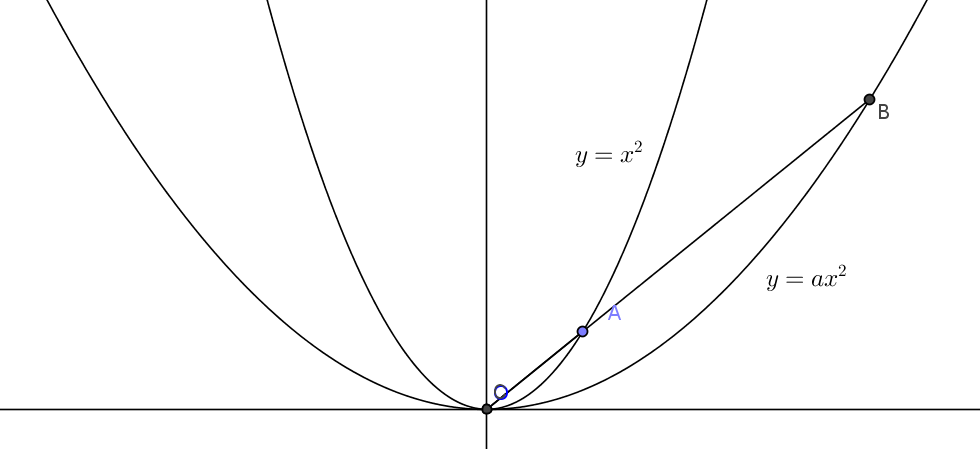
\includegraphics[width=0.7\textwidth]{problem_01}
\end{center}\medskip
\ep

\bp{02(cf. 1269)}
아래와 같이 이차함수 \(y=x^2\)의 그래프 위의 점 \(A\)에 대하여 반직선 \(OA\) 위에 \(\overline{OA}:\overline{OB}=3:5\)가 되도록 점 \(B\)를 잡으면 \(y=ax^2\)의 그래프가 점 \(B\)를 지난다.
이때 상수 \(a\)의 값을 구하여라. (단, \(O\)는 원점)
\par\medskip
\begin{center}
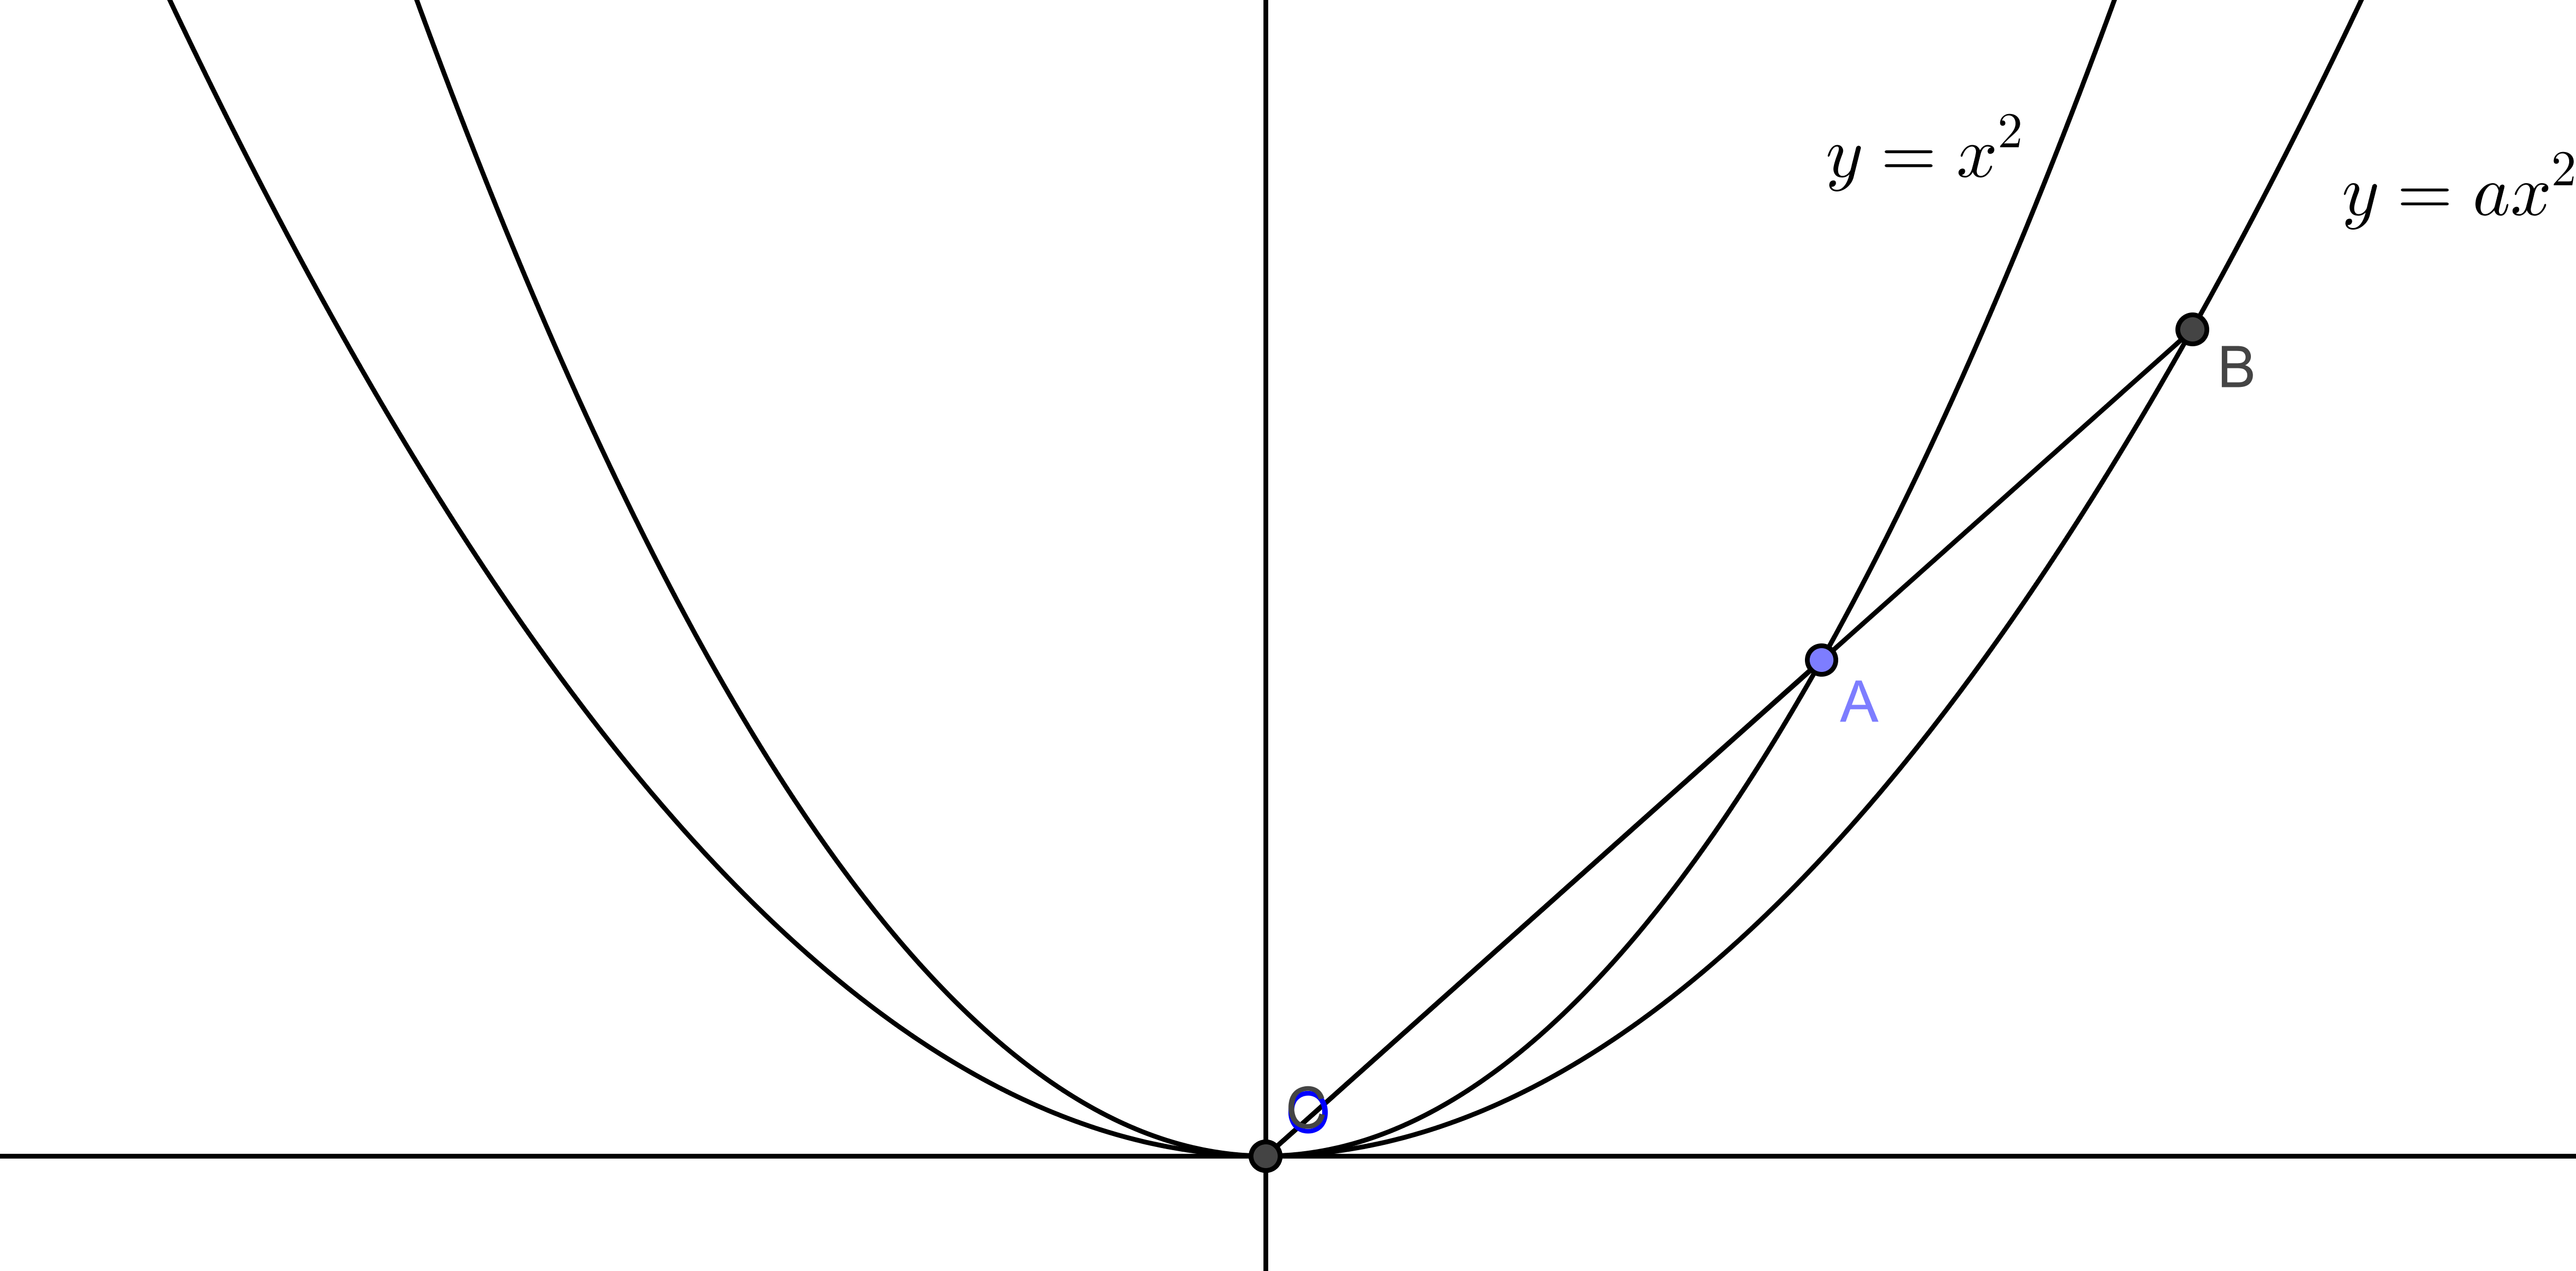
\includegraphics[width=0.7\textwidth]{problem_02}
\end{center}\medskip
\ep


\bp{03(cf. 1269)}
아래와 같이 이차함수 \(y=x^2\)의 그래프 위의 점 \(A\)에 대하여 반직선 \(OA\) 위에 \(\overline{OA}=3\overline{OB}\)가 되도록 점 \(B\)를 잡으면 \(y=ax^2\)의 그래프가 점 \(B\)를 지난다.
이때 상수 \(a\)의 값을 구하여라. (단, \(O\)는 원점)
\par\medskip
\begin{center}
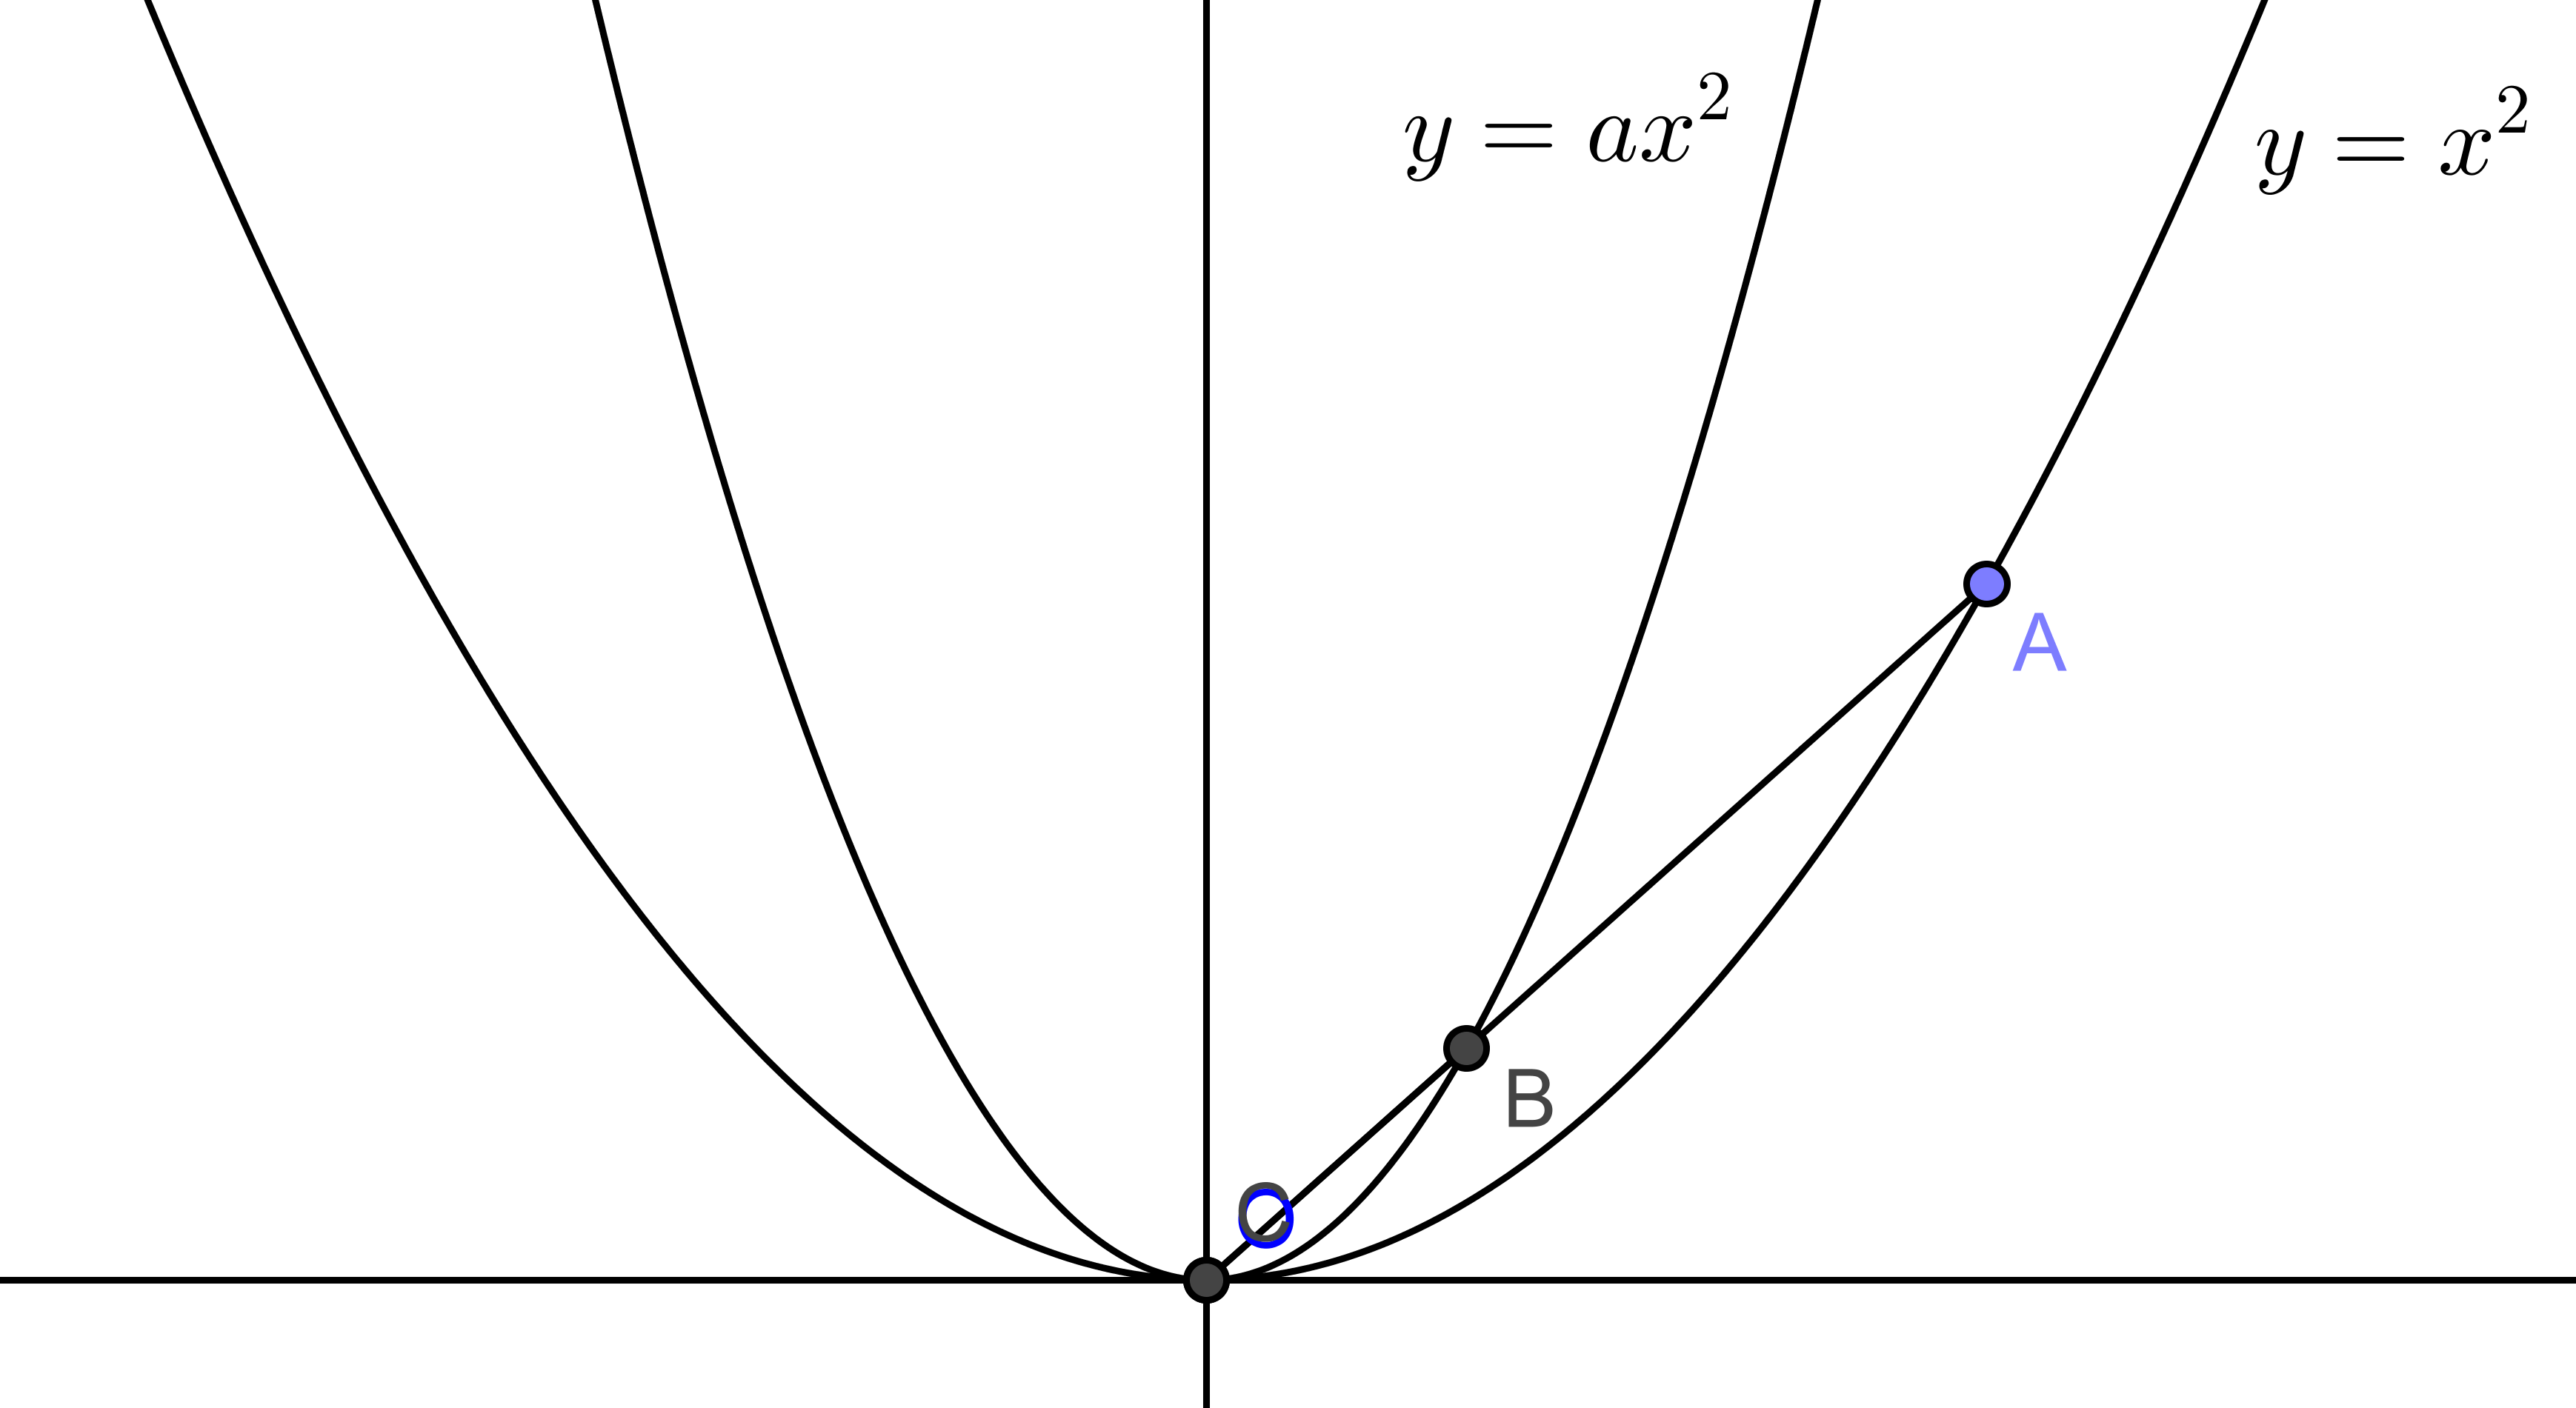
\includegraphics[width=0.7\textwidth]{problem_03}
\end{center}\medskip
\ep

\bp{04(cf. 1285)}
아래와 같이 두 이차함수 \(y=2x^2-18\), \(y=a(x-p)^2\)의 그래프가 서로의 꼭짓점을 지난다.
이 때 상수 \(a\), \(p\)에 대하여 \(a-p\)의 값을 구하여라. (단, \(p>0\))
\par\medskip
\begin{center}
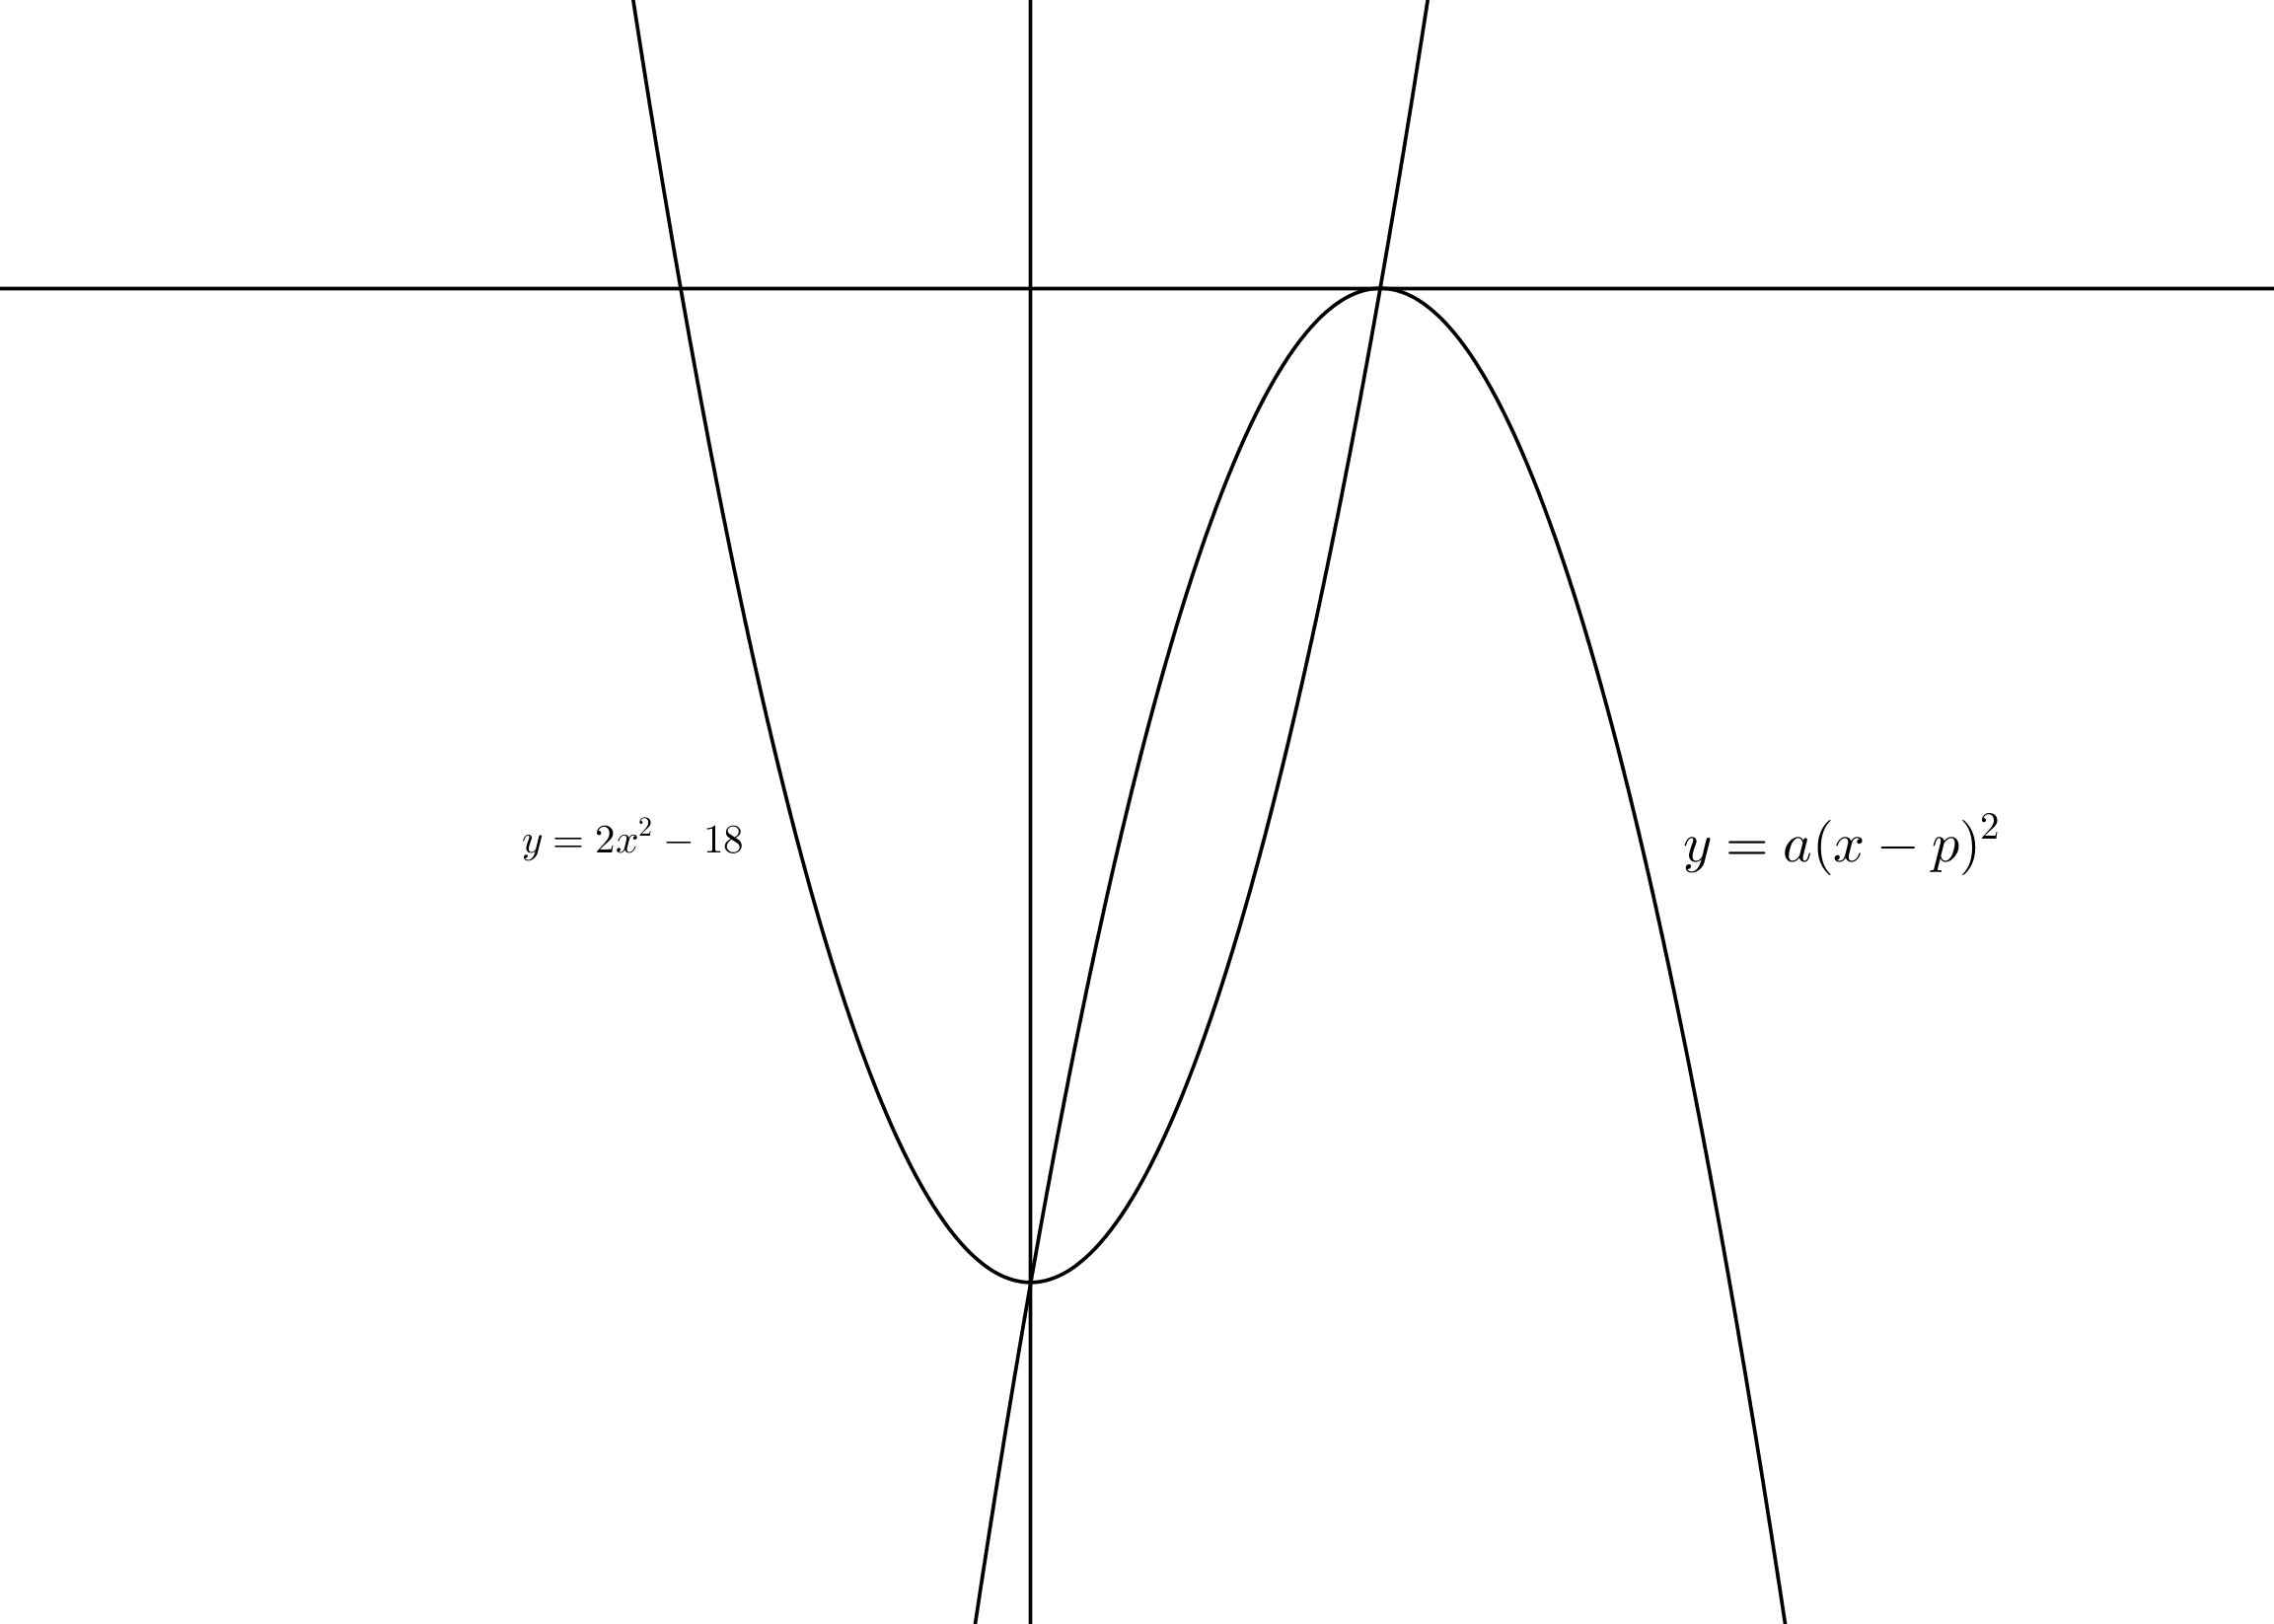
\includegraphics[width=0.5\textwidth]{problem_04}
\end{center}\medskip
\ep

\bp{05(cf. 1285)}
아래와 같이 두 이차함수 \(y = x^2\), \(y=ax^2+bx+c\)의 그래프가 서로의 꼭짓점을 지난다.
또 \(y=ax^2+bx+c\)는 \((7,-7)\)을 지날 때 \(a+b+c\)의 값을 구하여라.
\par\medskip
\begin{center}
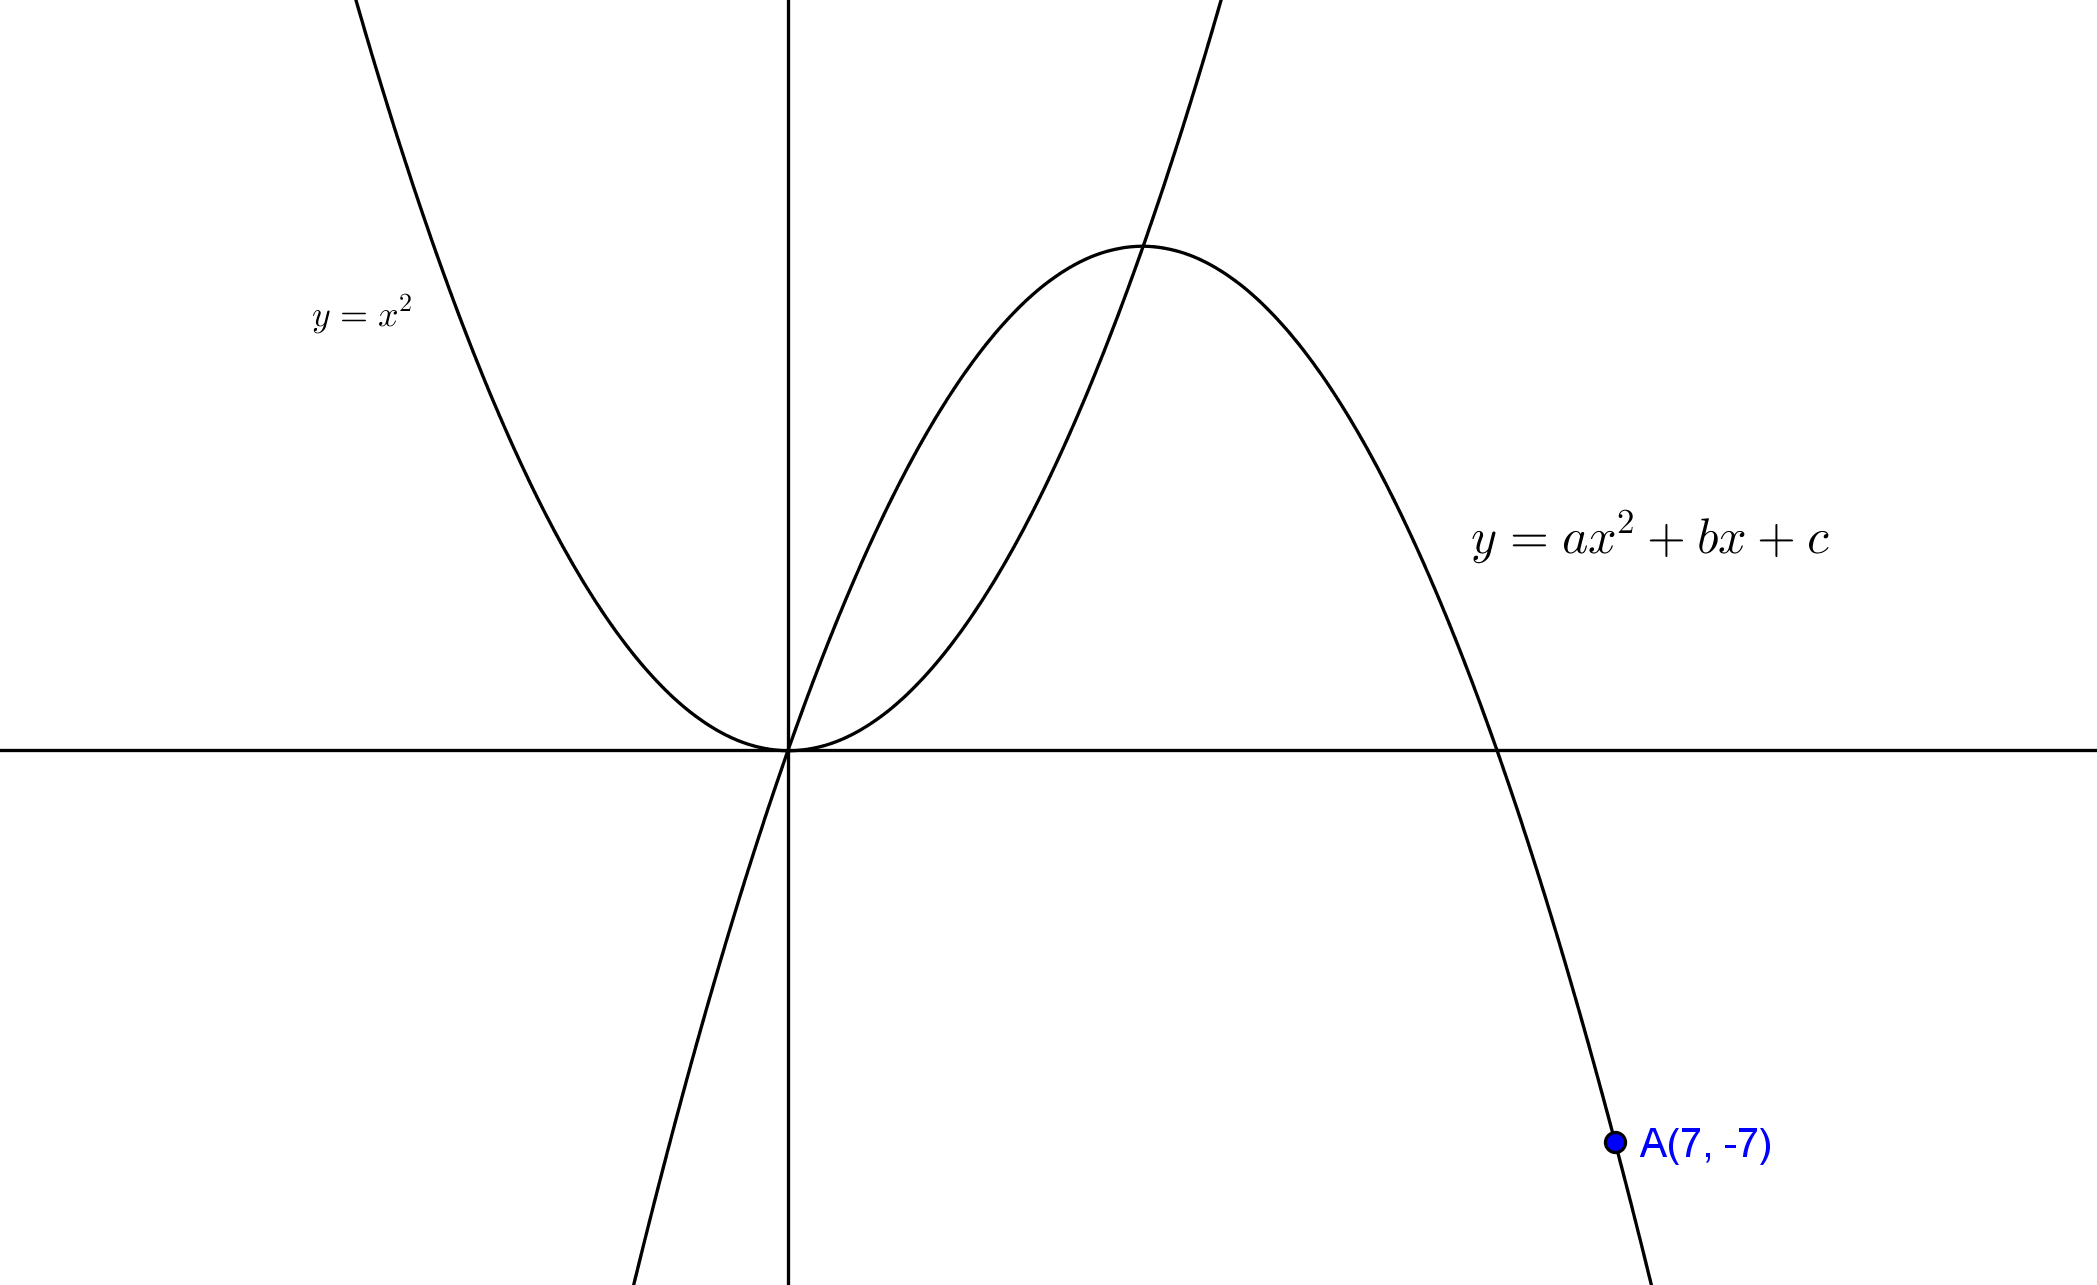
\includegraphics[width=0.5\textwidth]{problem_05}
\end{center}\medskip
\ep

\bp{06(cf. 1285)}
아래와 같이 두 이차함수 \(y = x^2 - 2x + 3\), \(y=ax^2+bx+c\)의 그래프가 서로의 꼭짓점을 지난다.
또 \(y=ax^2+bx+c\)는 \((8,8)\)을 지날 때 \(a+b+c\)의 값을 구하여라.
\par\medskip
\begin{center}
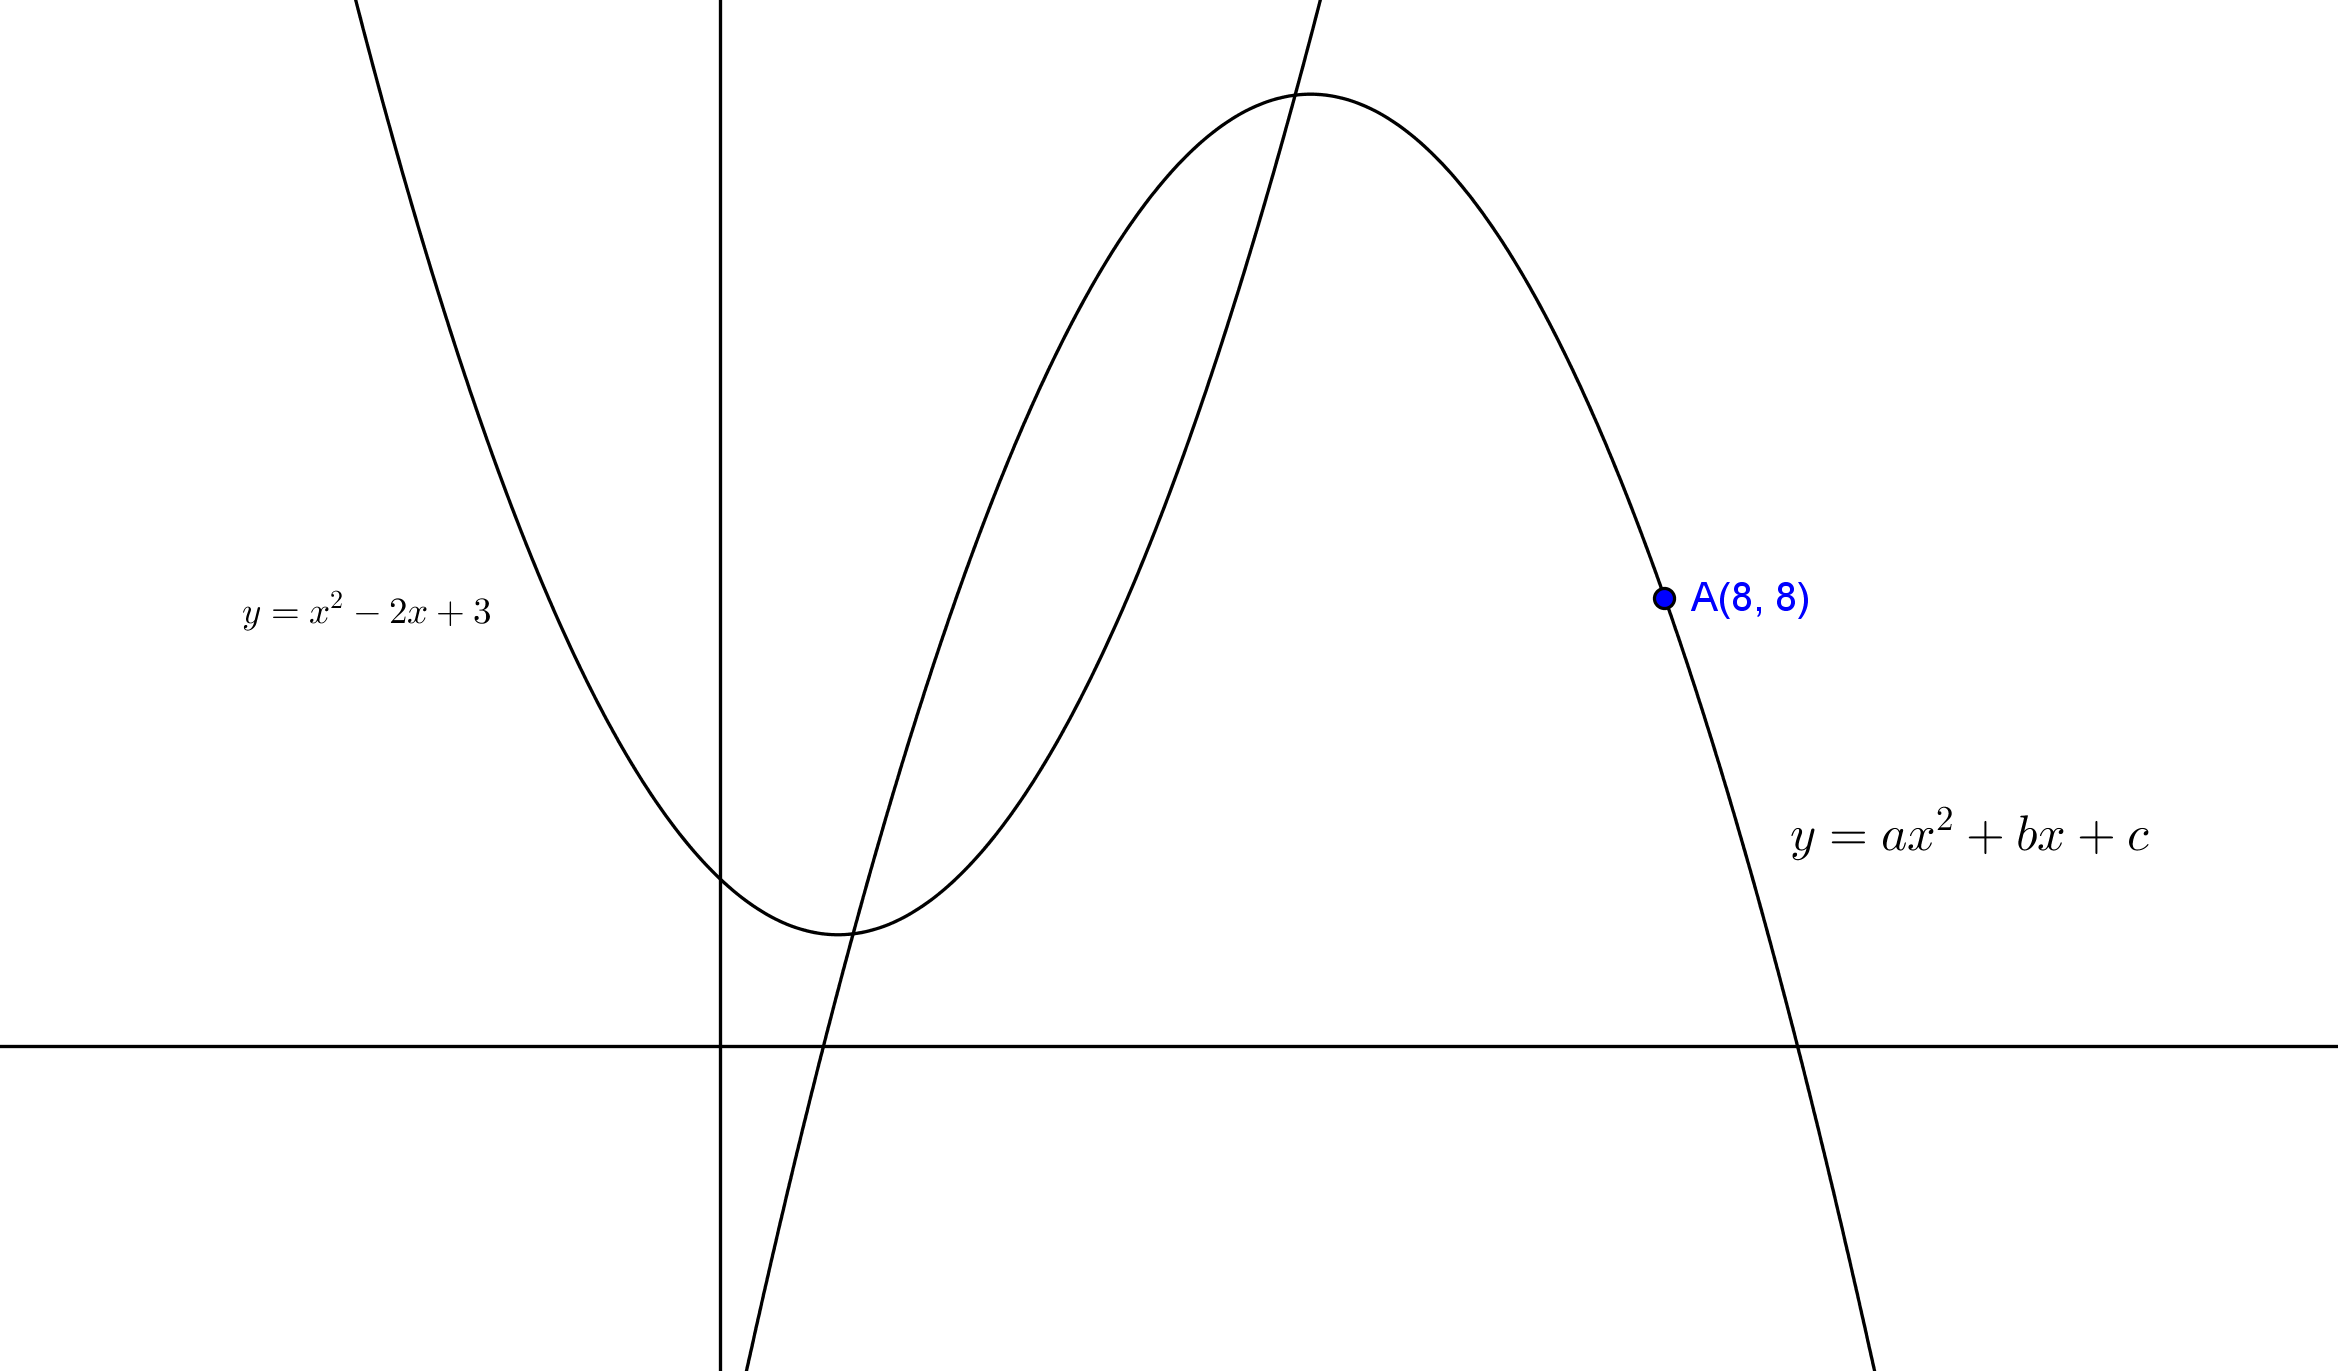
\includegraphics[width=0.5\textwidth]{problem_06}
\end{center}\medskip
\ep

\bp{07(cf. 1286)}
아래 그림은 두 이차함수 \(y=x^2\)과 \(y=2x^2-1\)이다.
색칠한 부분의 넓이를 구하여라.
\par\medskip
\begin{center}
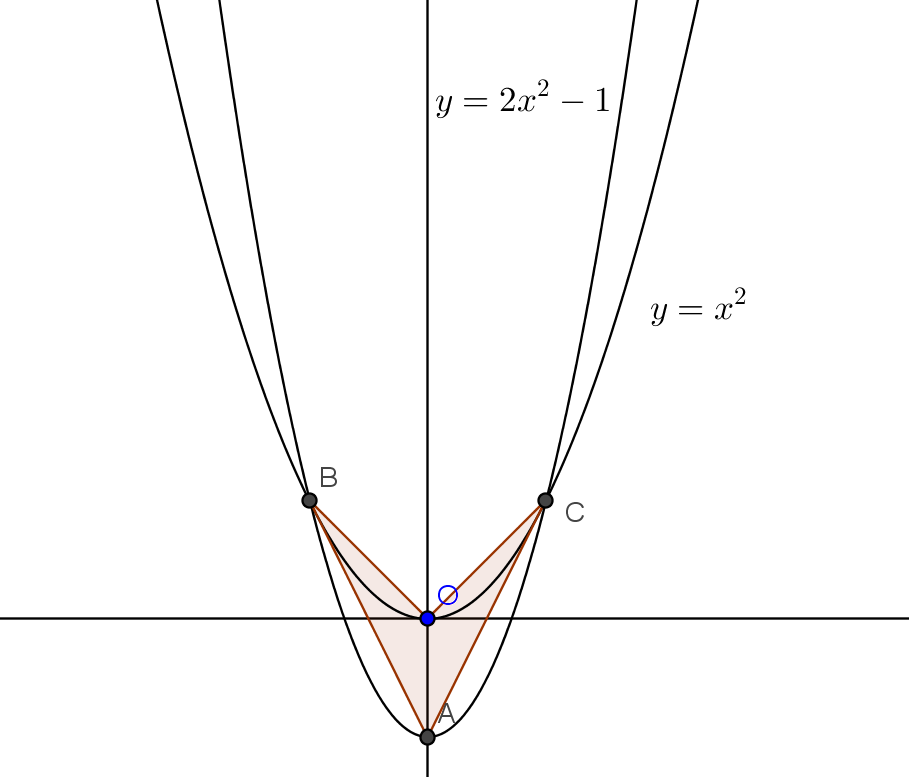
\includegraphics[width=0.5\textwidth]{problem_07}
\end{center}\medskip
\ep

\bp{08(cf. 1286)}
아래 그림은 두 이차함수 \(y=2x^2\)과 \(y=-3x^2+5\)이다.
색칠한 부분의 넓이를 구하여라.
\par\medskip
\begin{center}
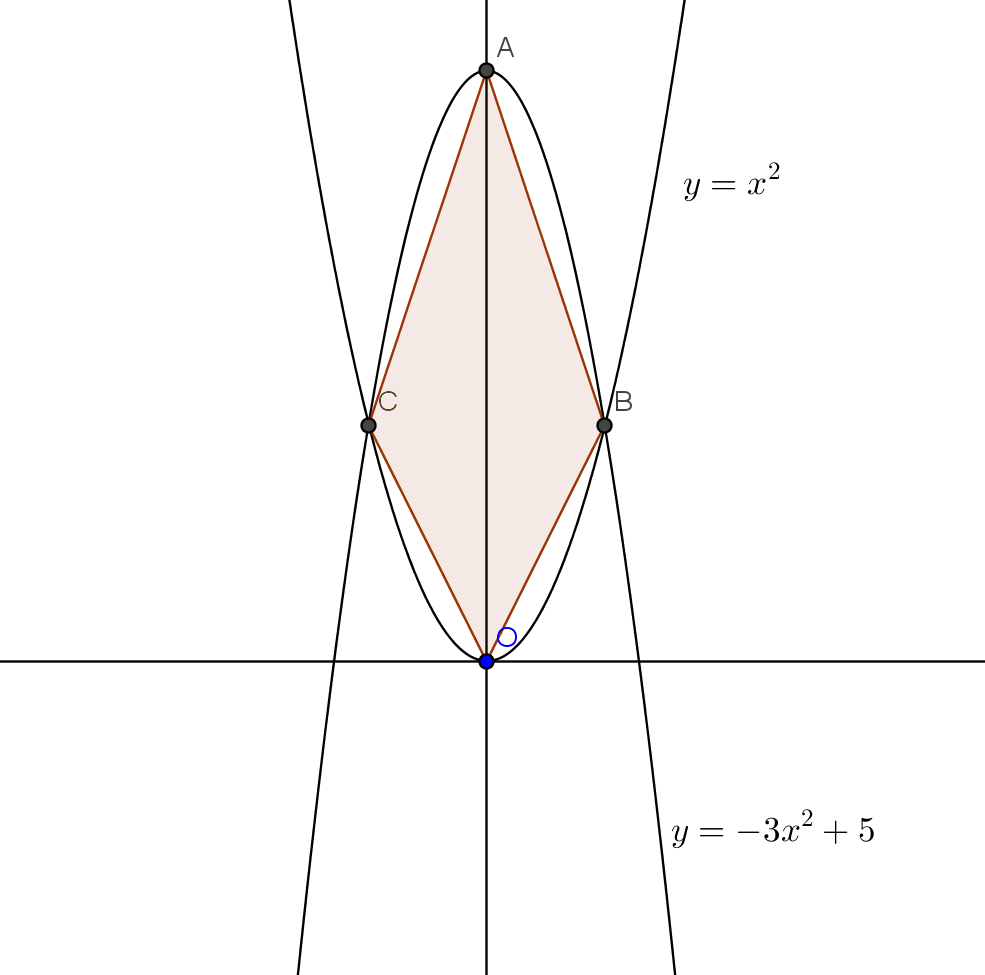
\includegraphics[width=0.5\textwidth]{problem_08}
\end{center}\medskip
\ep


\bp{09(cf. 1286)}
아래 그림은 두 이차함수 \(y=x^2\)과 \(y=-ax^2+9\)이다.
색칠한 부분의 넓이가 \(9\)가 되기 위한 \(a\)의 값은?
\par\medskip
\begin{center}
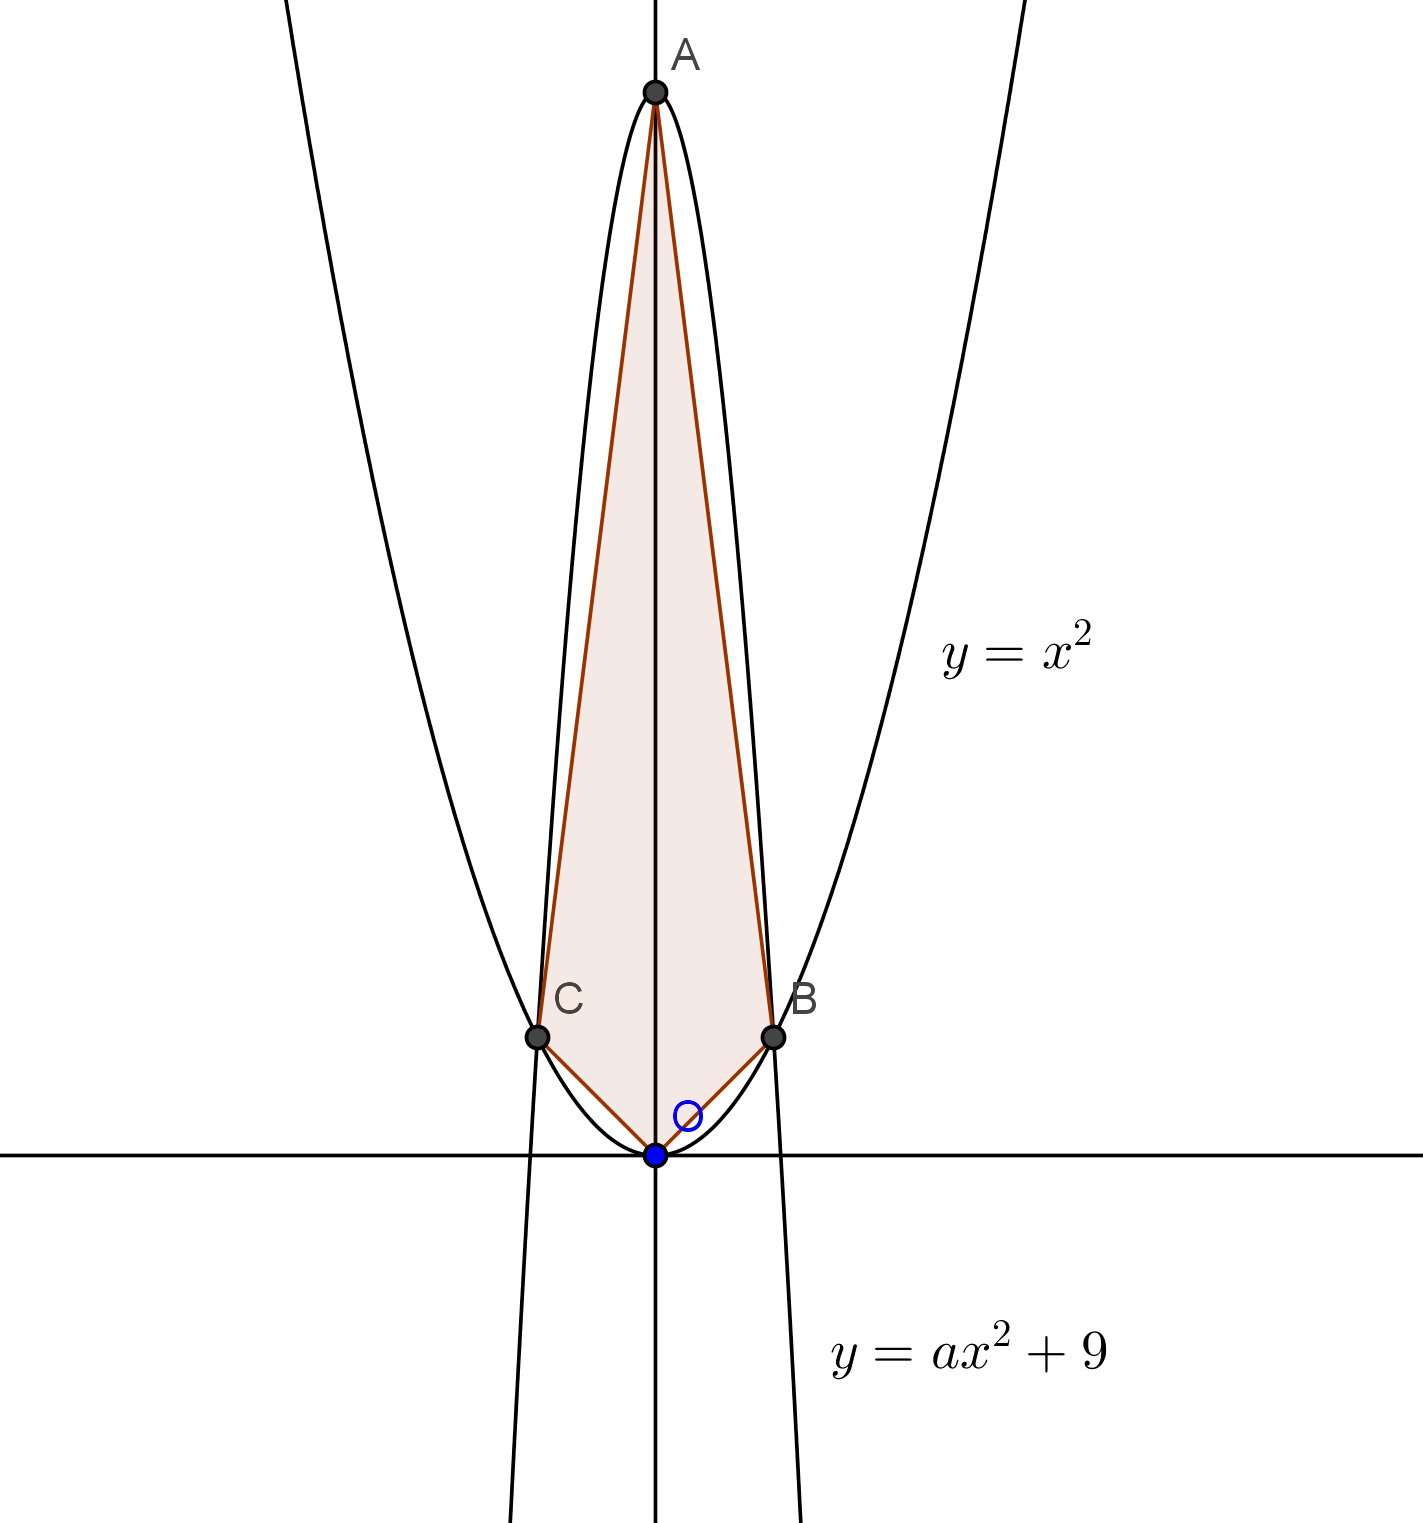
\includegraphics[width=0.5\textwidth]{problem_09}
\end{center}\medskip
\ep


\bp{10(cf. 1347)}
이차함수 \(y=ax^2+bx+c\)의 그래프가 다음과 같을 때 다음 중 옳은 것은?
\par\medskip
\begin{center}
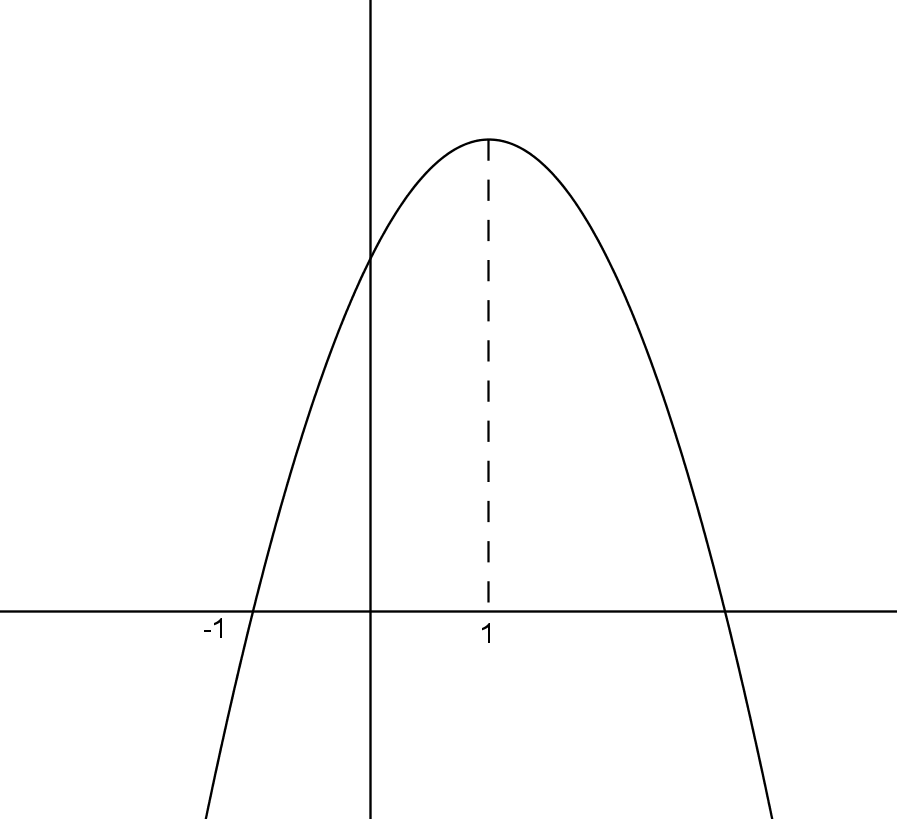
\includegraphics[width=0.5\textwidth]{problem_10}
\end{center}\medskip
\par
\noindent
\begin{inparaenum}
\item[①]
\(ab>0\)
\tab\item[②]
\(\frac ac>0\)
\tab\item[③]
\(b<0\)
\tab\item[④]
\(a+b+c<0\)
\tab\item[⑤]
\(a-b+c=0\)
\end{inparaenum}
\ep

\bp{11(cf. 1347)}
이차함수 \(y=ax^2+bx+c\)의 그래프가 다음과 같을 때 다음 중 옳은 것은?
\par\medskip
\begin{center}
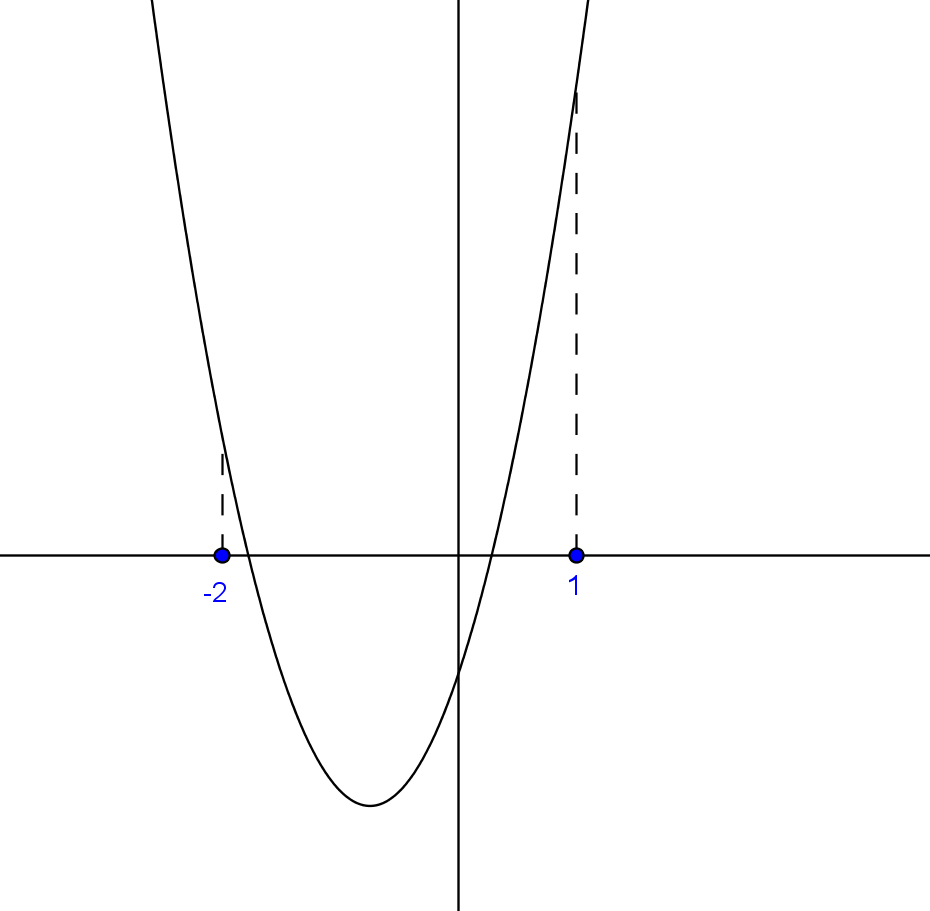
\includegraphics[width=0.5\textwidth]{problem_11}
\end{center}\medskip
\par
\noindent
\begin{inparaenum}
\item[①]
\(ab>0\)
\tab\item[②]
\(\frac ac>0\)
\tab\item[③]
\(b<0\)
\tab\item[④]
\(a+b+c<0\)
\tab\item[⑤]
\(4a-2b+c=0\)
\end{inparaenum}
\ep

\bp{12}
\(1\le x\le 3\)일 때\(y=x^2-4x\)의 최댓값, 최솟값을 더한 값은?
\ep

\bp{13}
\(-2\le x\le 3\)일 때\(y=-x^2+2x+2\)의 최댓값, 최솟값을 더한 값은?
\ep

\bp{14}
\(1\le x\le 2\)일 때\(y=3x^2+18x+1\)의 최댓값, 최솟값을 더한 값은?
\ep

\bp{15}
\(-1\le x\le 2\)일 때\(y=-x^2+4x+1\)의 최댓값, 최솟값을 더한 값은?
\ep

\bp{16(cf. 수학익힘책)}
아래와 같은 그림에서 이차함수 \(y=ax^2\)이 직사각형 \(ABCD\)의 둘레와의 교점이 두 개이기 위한 \(a\)의 범위는? (단 \(A=(1,1)\), \(B=(3,1)\), \(C=(3,4)\), \(D=(1,4)\))
\par\medskip
\begin{center}
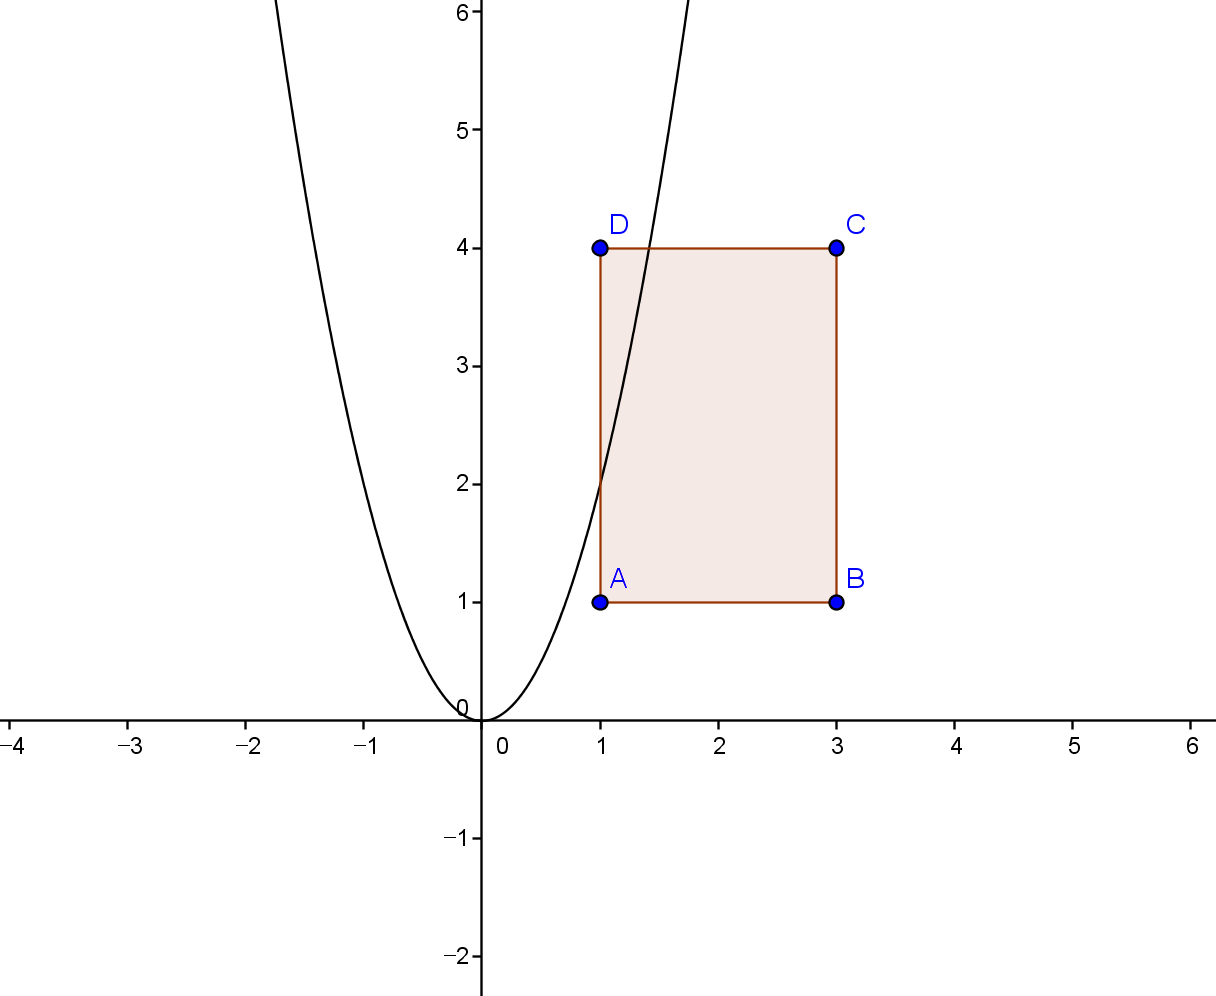
\includegraphics[width=0.5\textwidth]{problem_16}
\end{center}\medskip
\par
\ep

\bp{17(cf. 수학익힘책)}
아래와 같은 정사각형 \(ABCD\)에서 \(\overline{BD}\)의 길이는 \(12\)이다.
\(\overline{AB}\) 위의 한 점 \(E\)에 대해,\(E\)를 지나고 \(\overline{AC}\)와 평행한 직선이 \(\overline{BC}\)와 만나는 점을 \(F\), \(F\)를 지나고 \(\overline{BD}\)와 평행한 직선이 \(\overline{CD}\)와 만나는 점을 \(G\), \(G\)를 지나고 \(\overline{AC}\)와 평행한 직선이 \(\overline{AD}\)와 만나는 점을 \(H\)라고 하자.
직사각형 \(EFGH\)의 넓이가 최대가 될 때 이 직사각형의 둘레는?
\par\medskip
\begin{center}
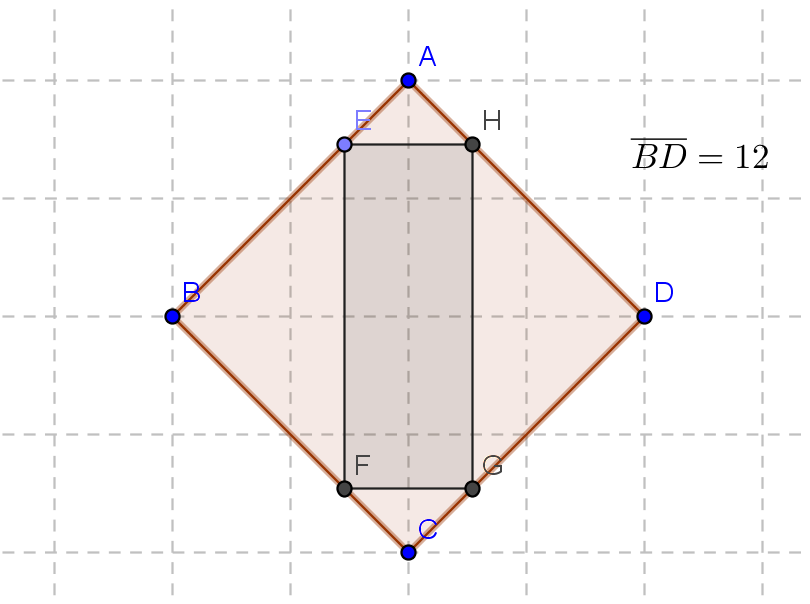
\includegraphics[width=0.5\textwidth]{problem_17}
\end{center}\medskip
\par
\ep

\bp{18*(cf. 1462)}
이차함수 \(y=x^2+4ax+8a+5\)의 최솟값을 \(m\)이라고 할 때 \(m\)의 최대값은?
\ep

\bp{19(cf. 1506)}
아래 그림과 같이 점 \(A\)는 이차함수 \(y = x^2 + 3x + 3\)의 그래프 위에 있고 \(B\)는 일차함수 \(y=x+1\)의 그래프 위에 있으며 두 점의 \(x\)좌표는 일치한다. 선분 \(\overline{AB}\)의 최솟값은?
\par\medskip
\begin{center}
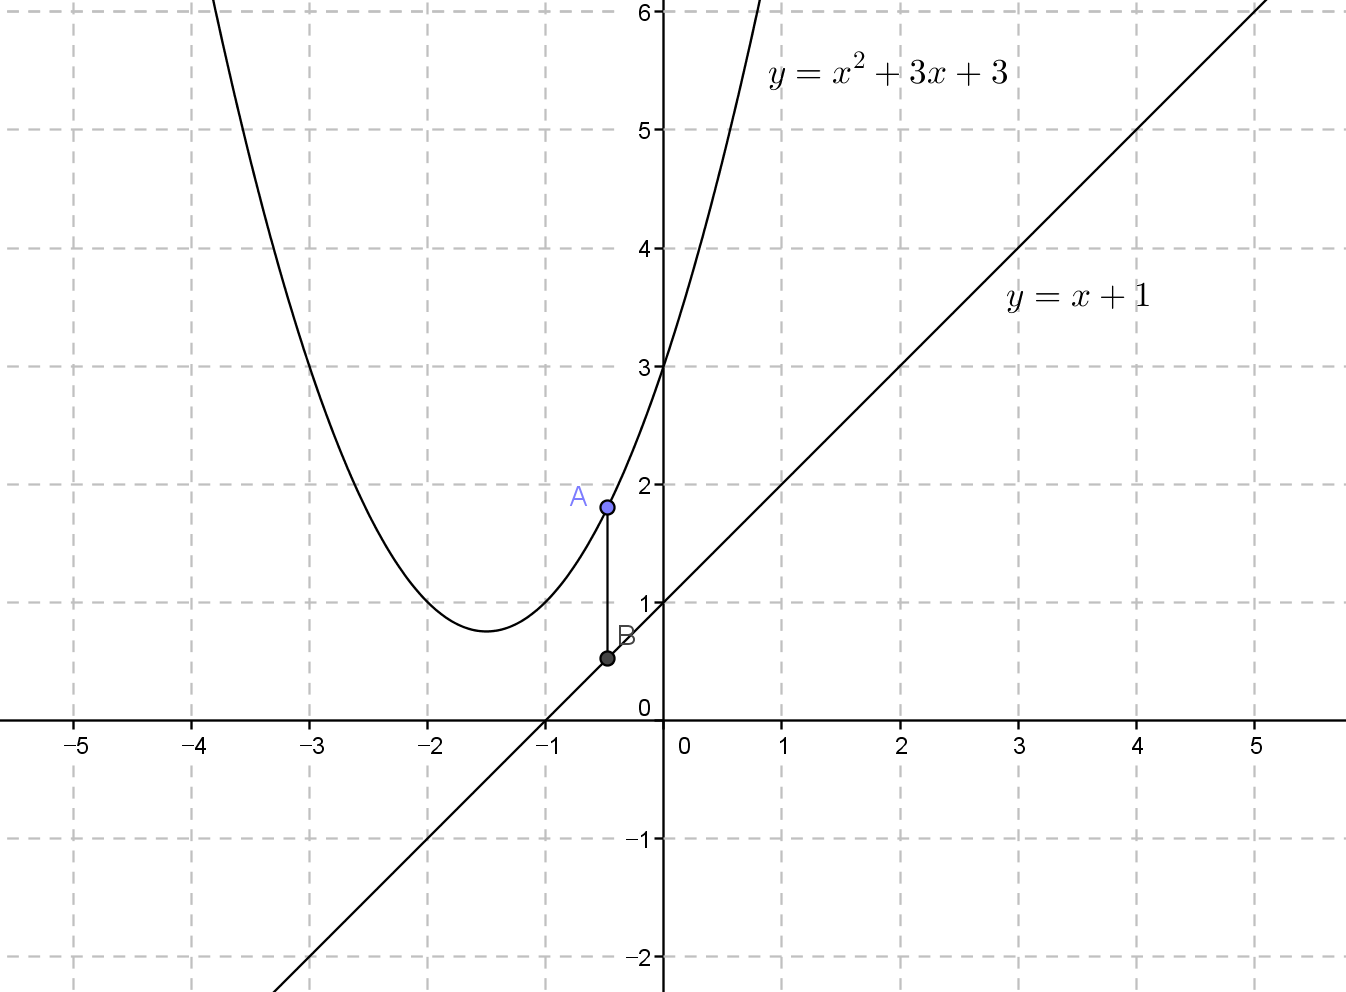
\includegraphics[width=0.5\textwidth]{problem_19}
\end{center}\medskip
\par
\ep

\bp{20(cf. 1506)}
아래 그림과 같이 점 \(A\)는 이차함수 \(y = x^2 +1\)의 그래프 위에 있고 \(B\)는 이차함수 \(y=-x^2+4x-3\)의 그래프 위에 있으며 두 점의 \(x\)좌표는 일치한다. 선분 \(\overline{AB}\)의 최솟값은?
\par\medskip
\begin{center}
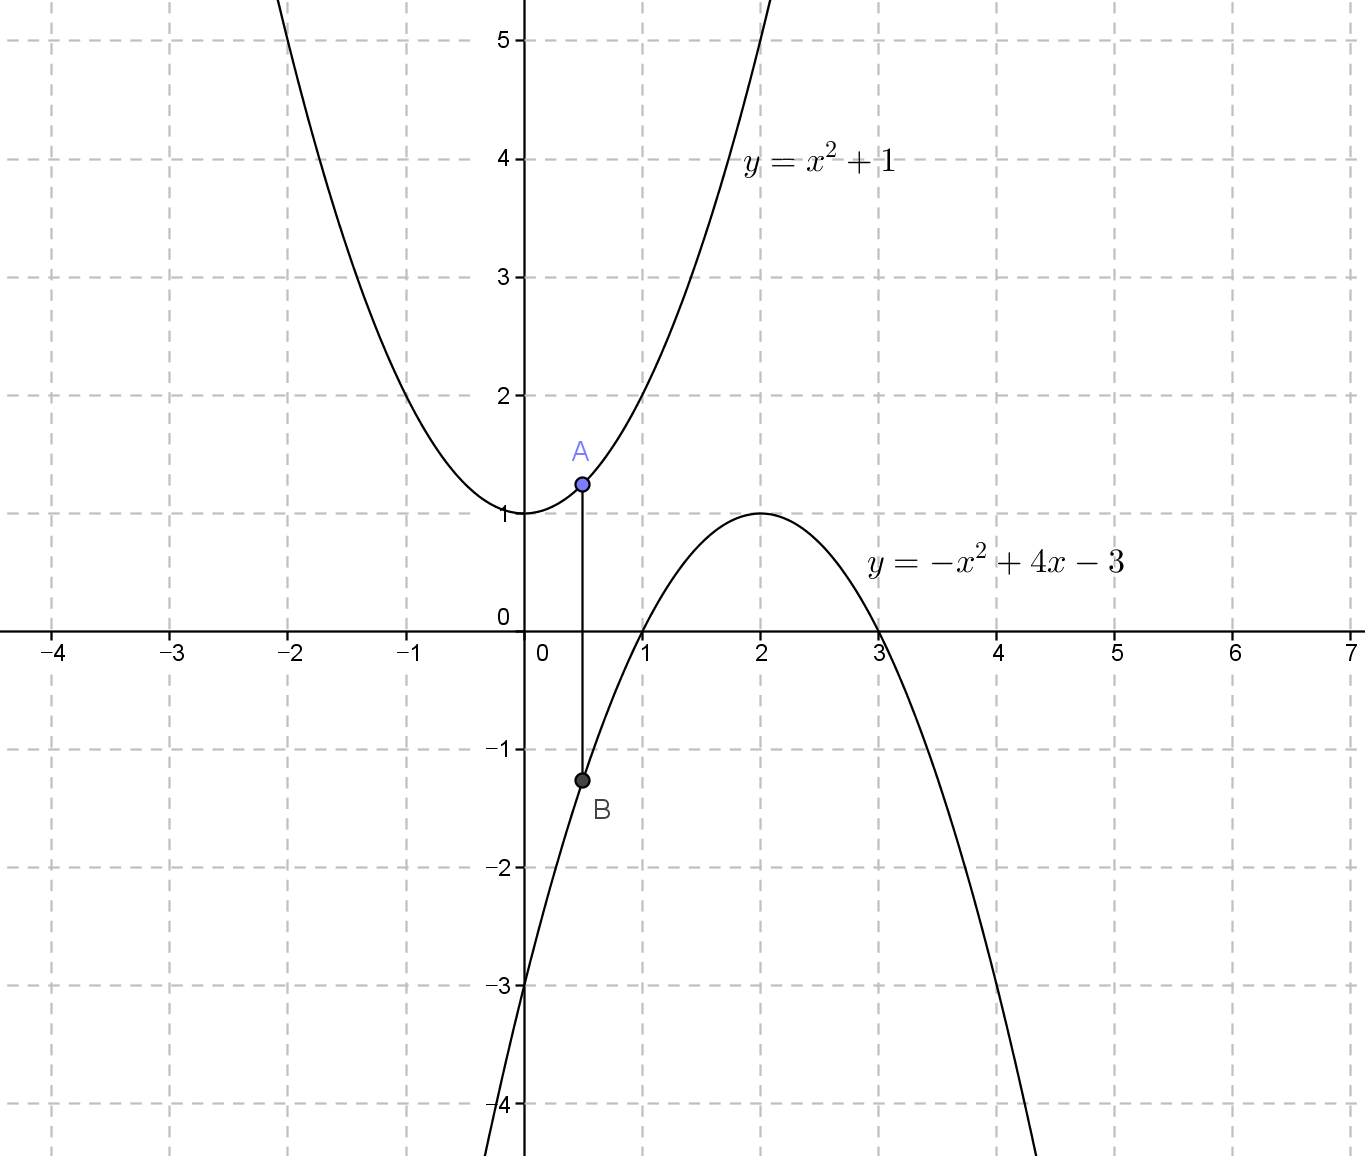
\includegraphics[width=0.5\textwidth]{problem_20}
\end{center}\medskip
\par
\ep
%
%\bp{21(cf. 1506)}
%아래 그림과 같이 점 \(A\)는 이차함수 \(y = x^2 +1\)의 그래프 위에 있고 \(B\)는 이차함수 \(y=-x^2+4x-3\)의 그래프 위에 있으며 두 점의 \(x\)좌표는 일치한다. 선분 \(\overline{AB}\)의 최솟값은?
%\par\medskip
%\begin{center}
%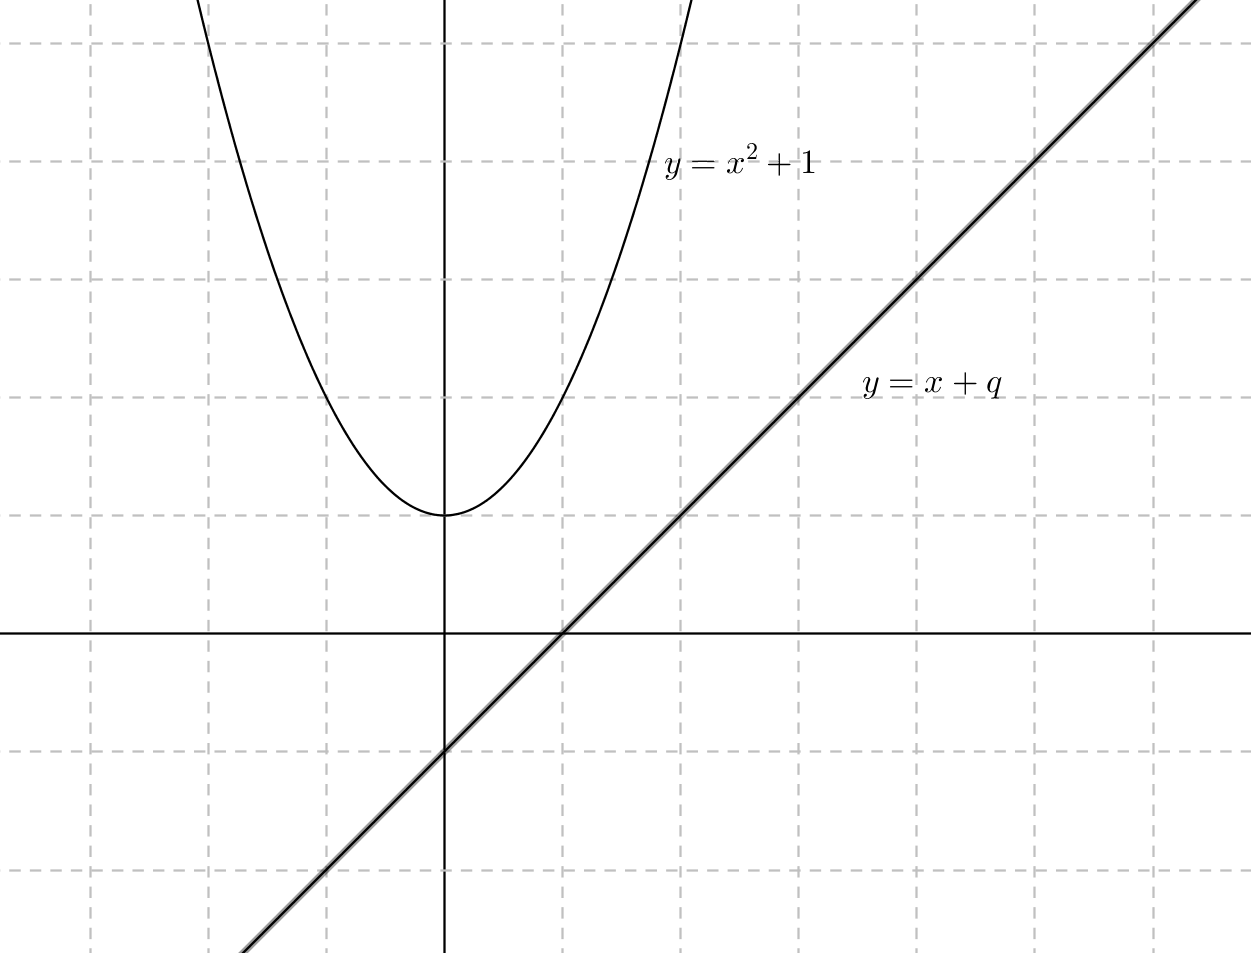
\includegraphics[width=0.5\textwidth]{problem_21}
%\end{center}\medskip
%\par
%\ep

\bp{21(cf. 1506)}
아래 그림과 같이 이차함수 \(y = x^2 + 3x + 3\)의 그래프와 일차함수 \(y=x+q\)의 그래프가 만나지 않기 위한 \(q\)값의 범위는?
\par\medskip
\begin{center}
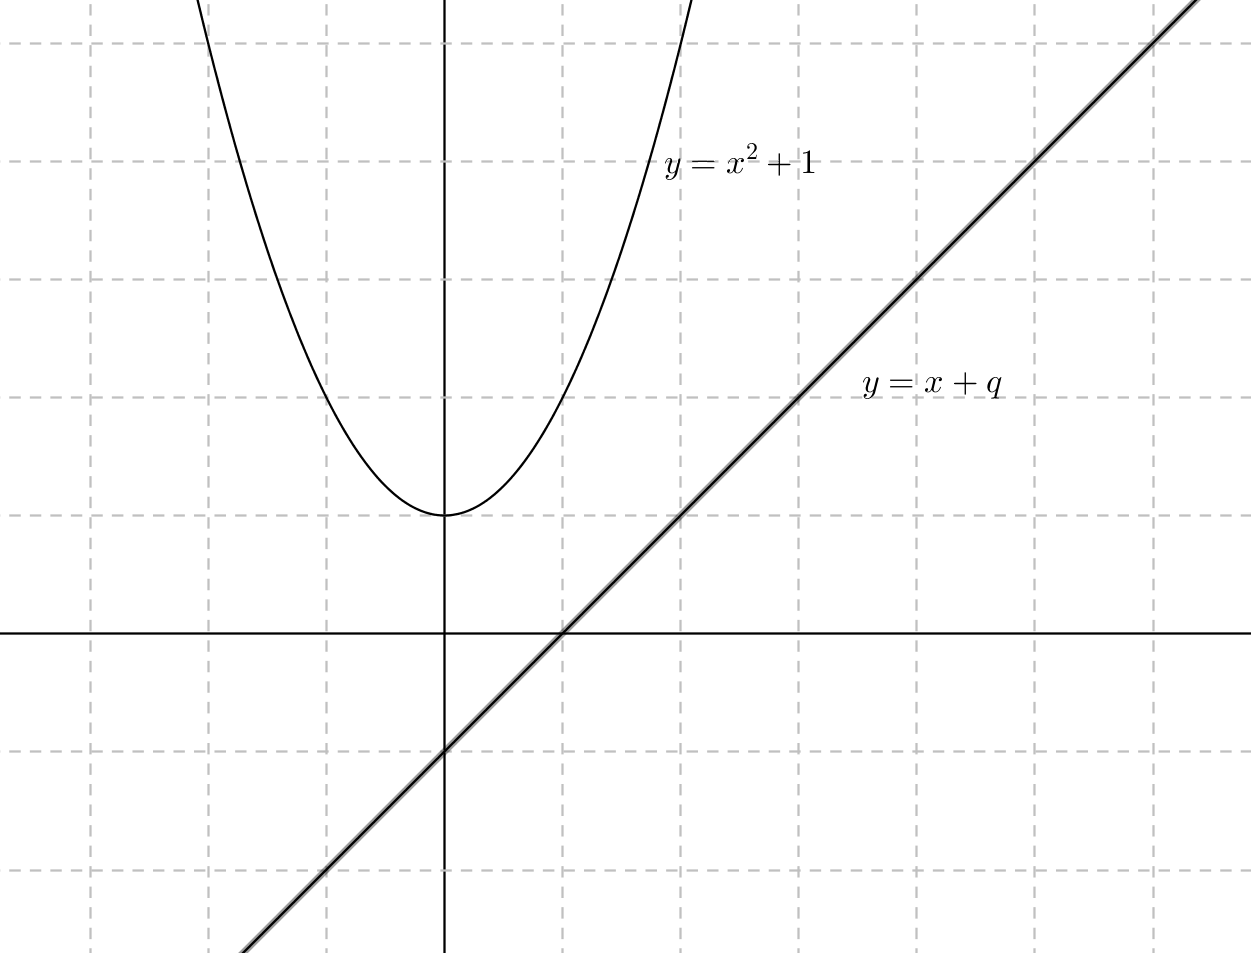
\includegraphics[width=0.5\textwidth]{problem_21}
\end{center}\medskip
\par
\ep

\bp{22(cf. 1506)}
아래 그림과 같이 이차함수 \(y = x^2 +q\)의 그래프와 이차함수 \(y=-x^2+4x-3\)의 그래프가 만나지 않기 위한 \(q\)값의 범위는?
\par\medskip
\begin{center}
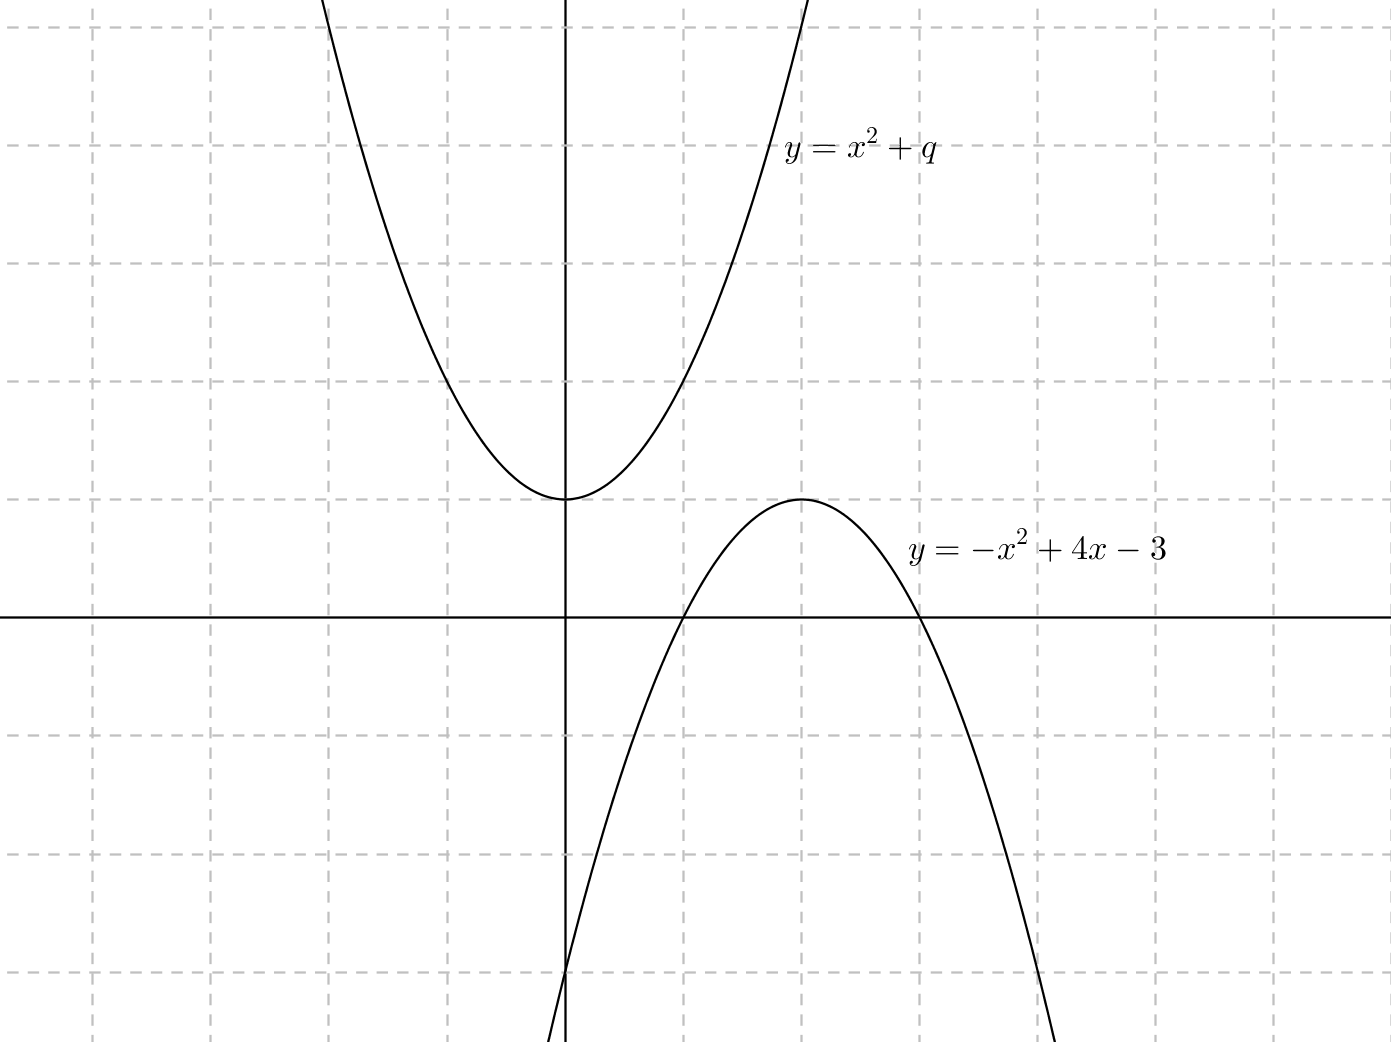
\includegraphics[width=0.5\textwidth]{problem_22}
\end{center}\medskip
\par
\ep

\newpage
\section*{답}
01 : \(\frac14\)\\
02 : \(0.6\)\\
03 : \(3\)\\
04 : \(-1\)\\
05 : \(5\)\\
06 : \(1\)\\
07 : \(1\)\\
08 : \(5\)\\
09 : \(8\)\\
10 : ⑤\\
11 : ①\\
12 : \(-7\)\\
13 : \(-3\)\\
14 : \(71\)\\
15 : \(1\)\\
16 : \(\frac19<a<4\)\\
17 : \(24\) \\
18 : \(9\)\\
19 : \(1\)\\
20 : \(2\)\\
21 : \(q<2\)\\
22 : \(q>-1\).

\end{document}